\section{Scene}

Scena sadrži sve objekte igre koji se koriste. Scena nam može služiti za kreiranje izbornika, ukoliko igra ima više levela, svaki level će se nalaziti u svojoj sceni. Preko scene uređujemo okolinu, postavljamo objekte i prepreke. Scena zapravo sve sklopljene elemente pretvara u jedan sadržaj. 
\subsection{Main menu}
Ovo je početna scena u igri. Scena sadrži platno sa tekstom i dva botuna te objektom "plane" na kojega je zaljepljena slika radi boljeg ugođaja. 

\begin{center}
	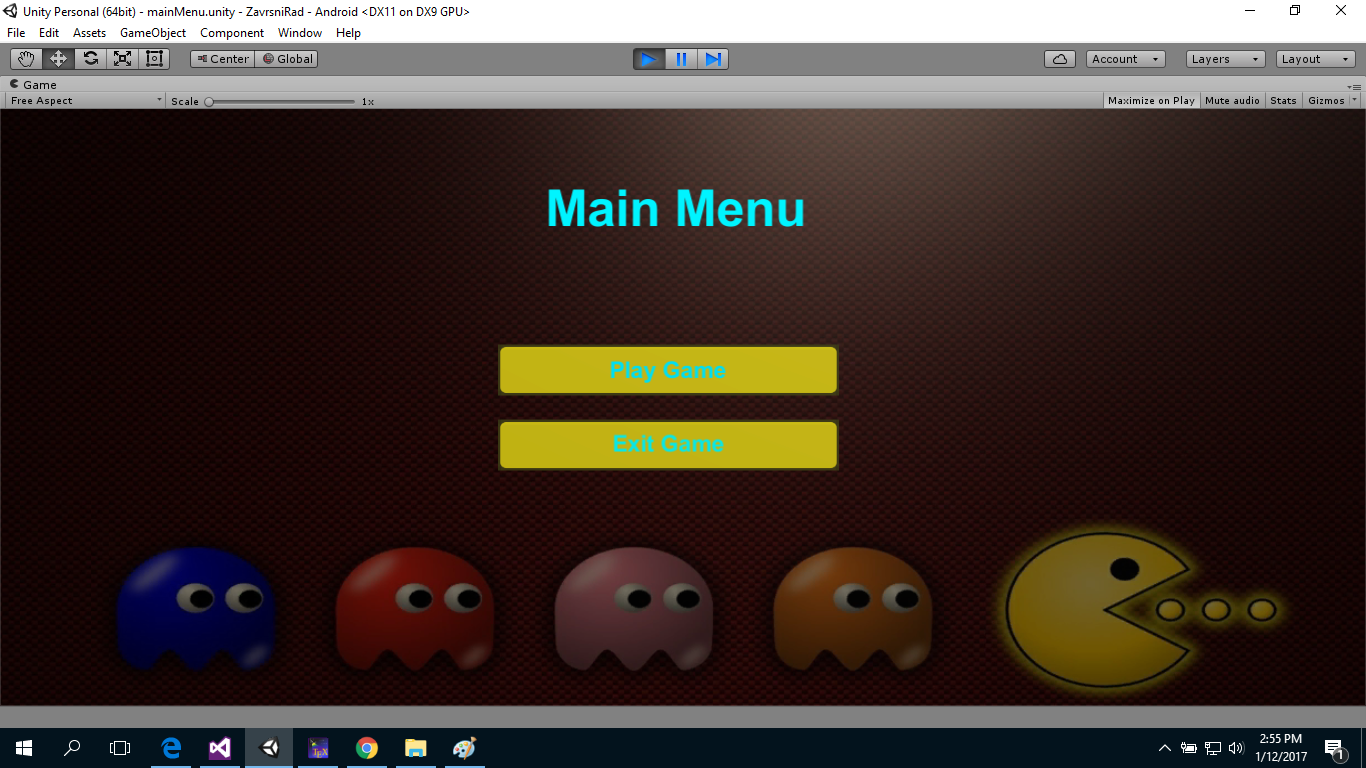
\includegraphics[scale=0.20]{scena1.png}
	
	Slika 3: Scena "Main Menu"
\end{center}




\subsection{Game}
"Game" je glavna scena na koju korisnik dolazi pritiskom botuna "Play" na "Main Menu" sceni. Sadrži sve doli napisane objekte i njihove komponente. Također sadrži i platno koje se pojavljuje po potrebi i preko kojeg se može vratiti na početnu scenu.
\begin{center}
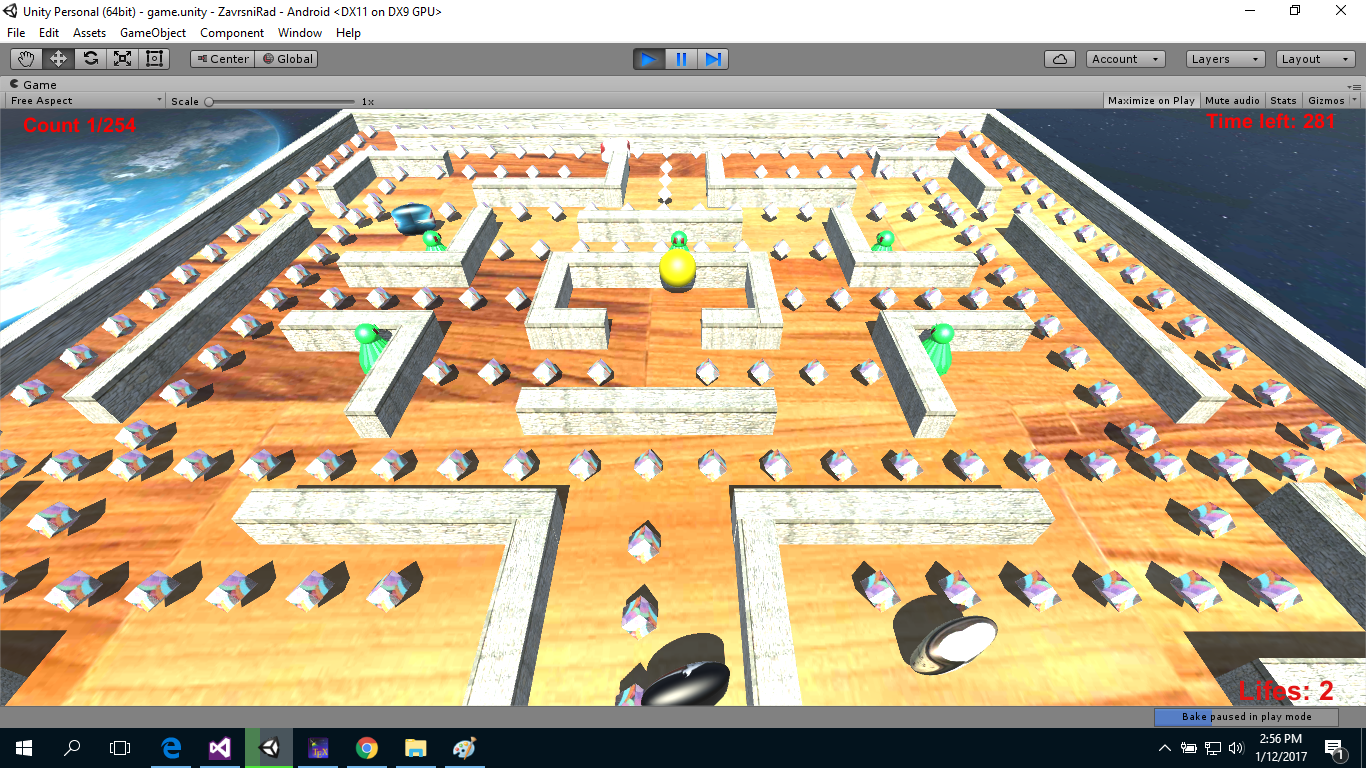
\includegraphics[scale=0.20]{scena2.png}

Slika 4: Scena "Game"
\end{center}
